\documentclass[jocse]{jocseart}

\usepackage{booktabs}
\usepackage[utf8]{inputenc}
\usepackage[english]{babel}

% Copyright
\setcopyright{jocsecopyright}
\jocseDOI{10.22369/issn.2153-4136/x/x/x }

\pagestyle{plain}
\pagenumbering{gobble}

\usepackage{cleveref}
\usepackage{todonotes}
\usepackage{graphicx}
\graphicspath{{./fig/}}
\DeclareGraphicsExtensions{.png,.pdf,.jpg,.jpeg}

\newcommand{\jk}[1]{\todo[inline]{TODO: #1}}

\begin{document}
\title{One Year HPC Certification Forum in Retrospective}

\author{Julian Kunkel}
\affiliation{%
  \institution{University of Reading}
  \streetaddress{}
  \city{Reading}
  \state{United Kingdom}
  \postcode{}
}
\email{j.m.kunkel@reading.ac.uk}


\author{Kai Himstedt}
\author{Nathanael Hübbe}
\affiliation{%
  \institution{Universität Hamburg}
  \streetaddress{}
  \city{Hamburg}
  \state{Germany}
  \postcode{}
}

\author{Weronika Filinger}
\affiliation{%
  \institution{EPCC, The University of Edinburgh}
  \streetaddress{}
  \city{Edinburgh}
  \state{United Kingdom}
  \postcode{}
}

\author{Jean-Thomas Acquaviva}
\affiliation{%
  \institution{DDN}
  \streetaddress{}
  \city{Paris}
  \state{France}
  \postcode{}
}


\author{Anja Gerbes}
\affiliation{%
  \institution{Goethe-Universität}
  \streetaddress{}
  \city{Frankfurt am Main}
  \state{Germany}
  \postcode{}
}

\author{Lev Lafayette}
\affiliation{%
  \institution{University of Melbourne}
  \streetaddress{}
  \city{Melburne}
  \state{Australia}
  \postcode{}
}

\renewcommand{\shortauthors}{J. Kunkel et al.}


\begin{abstract}
  The HPC community has always considered the training of new and existing HPC practitioners to be of high importance to its growth.
  This diversification of HPC practitioners challenges the traditional training approaches, which are not able to satisfy the specific needs of users, often coming from non-traditionally HPC disciplines, and only interested in learning a particular set of competences.
  Challenges for HPC centres are to identify and overcome the gaps in users’ knowledge, while users struggle to identify relevant skills.

  With the HPC Certification Forum we aim to clearly categorize, define, and examine competences which brings benefit to all stakeholders involved in training.
  In this paper, we report the status and progress this independent body has made during the first year of its existence.
  Particularly, in various directions drafts of processes and prototypes have been generated to create a holistic ecosystem that will mature over this year.
\end{abstract}

%
% The code below should be generated by the tool at
% http://dl.acm.org/ccs.cfm
% Please copy and paste the code instead of the example below.
%
\begin{CCSXML}
\end{CCSXML}



\keywords{}

\maketitle

\section{Introduction}

There is a generally accepted set of skills and competencies necessary to efficiently use HPC resources.
This skill set depends on the role and domain of the practitioner but also on the available infrastructure of the center providing the computing resources.
For example, a scientist needing to run an application on a specific machine may need basic skills in Linux, MPI, environment modules, and knowledge about the batch scheduler, e.g., SLURM.
Understanding SLURM is a good example of a very fine-grained skill, indeed we can identify "resource management" as a generic skill that illustrates concepts across the rich variety of available resource managers.
Institutions which operate HPC systems typically offer regularly teaching events about general aspects of their supercomputer's hard- and software architecture and about the software environment around parallel programming and optimization.
The learning material provided by an HPC center, however, is geared to the special demands of the institutions they support and its specific HPC environment.
This content typically covers a small part of basic HPC skills which are necessary to use other HPC systems.
Moreover, they do not attest the users to have a certain competence.
Certificates are widely used in industry to attest certain knowledge but, so far, there is no similar approach for HPC training.

This article describes the current status of the certification program offered by the HPC Certification Forum by looking back for the one year of this independent body that curate the competences and aims to issue certificates for the users.
Our previous work described the evolution from the project that sparked the initial activity that lead to the independent body of the HPC Certification Forum \cite{TAHCPKHHSS19}.


\section{The HPC Certification Forum}

The HPC Certification Forum (HPCCF) has the role of a (virtual) central authority to curate and maintain a skill tree of competences, the creation of certificates, and examination of practitioners to attest certificates.
Moreover, the forum supports tools and an ecosystem around the competences.

HPC Certification Program

\jk{Integrate}

1) the definition and organization of fine-grained competences (skills);
2) the establishment of certificates and (online) exams that confirm that users possess a certain skill.
Note that the certification program does not regulate the content -- the definition of skills and certificates is separated from content creation.
This allows the re-use of existing content but also allows to create a new ecosystem in which HPC centers or commercial companies could offer the best teaching material.
Teaching material should be marked to indicated which skills it covers.
In the future, the program may provide means to register and reference existing content of third-parties allowing users to browse the skills and navigate to teaching material.
We assume that the collaboration of scientific institutions will complement each other in producing a rich variety of content for the different learning styles.



\section{Skill Organization}

The competences are organized in a tree that serves the purpose to organize and structure the skills from a coarse-grained to a fine-grained representation allowing users to browse the skill based on the semantics.
The root level of our current skill tree is shown in \Cref{skill-tree}.
The idea is that the skills from the root level provide an indication about their scope,
e.g., are they core knowledge, dealing with the usage of HPC environments, or about programming.
This should allow the user to rapidly drill into the skill representation.
The closer a skill is to the root, the more abstract it is defined, while leaf nodes cover the knowledge for the specific skill.


Within a single skill, there can also be multiple levels (basic, intermediate, expert level) building upon each other -- thus, we expect that practitioners acquire the lower levels before progressing to more complex levels.
The basic level should cover the most relevant aspect of the skill, i.e., needed by anyone that uses the skill, the intermediate level (used for common exceptional cases) and expert levels (used in special circumstances)  are needed only for a subset of users.
Typically, an institution has only few experts (if one at all).

As the tree serves the purpose to organize the skills, there can also be references from one branch to a skill in another.
This import allows to reuse the definitions of the skills while still allowing users to navigate the tree according to the semantics.

\begin{figure*}[tb!]
	\centering
	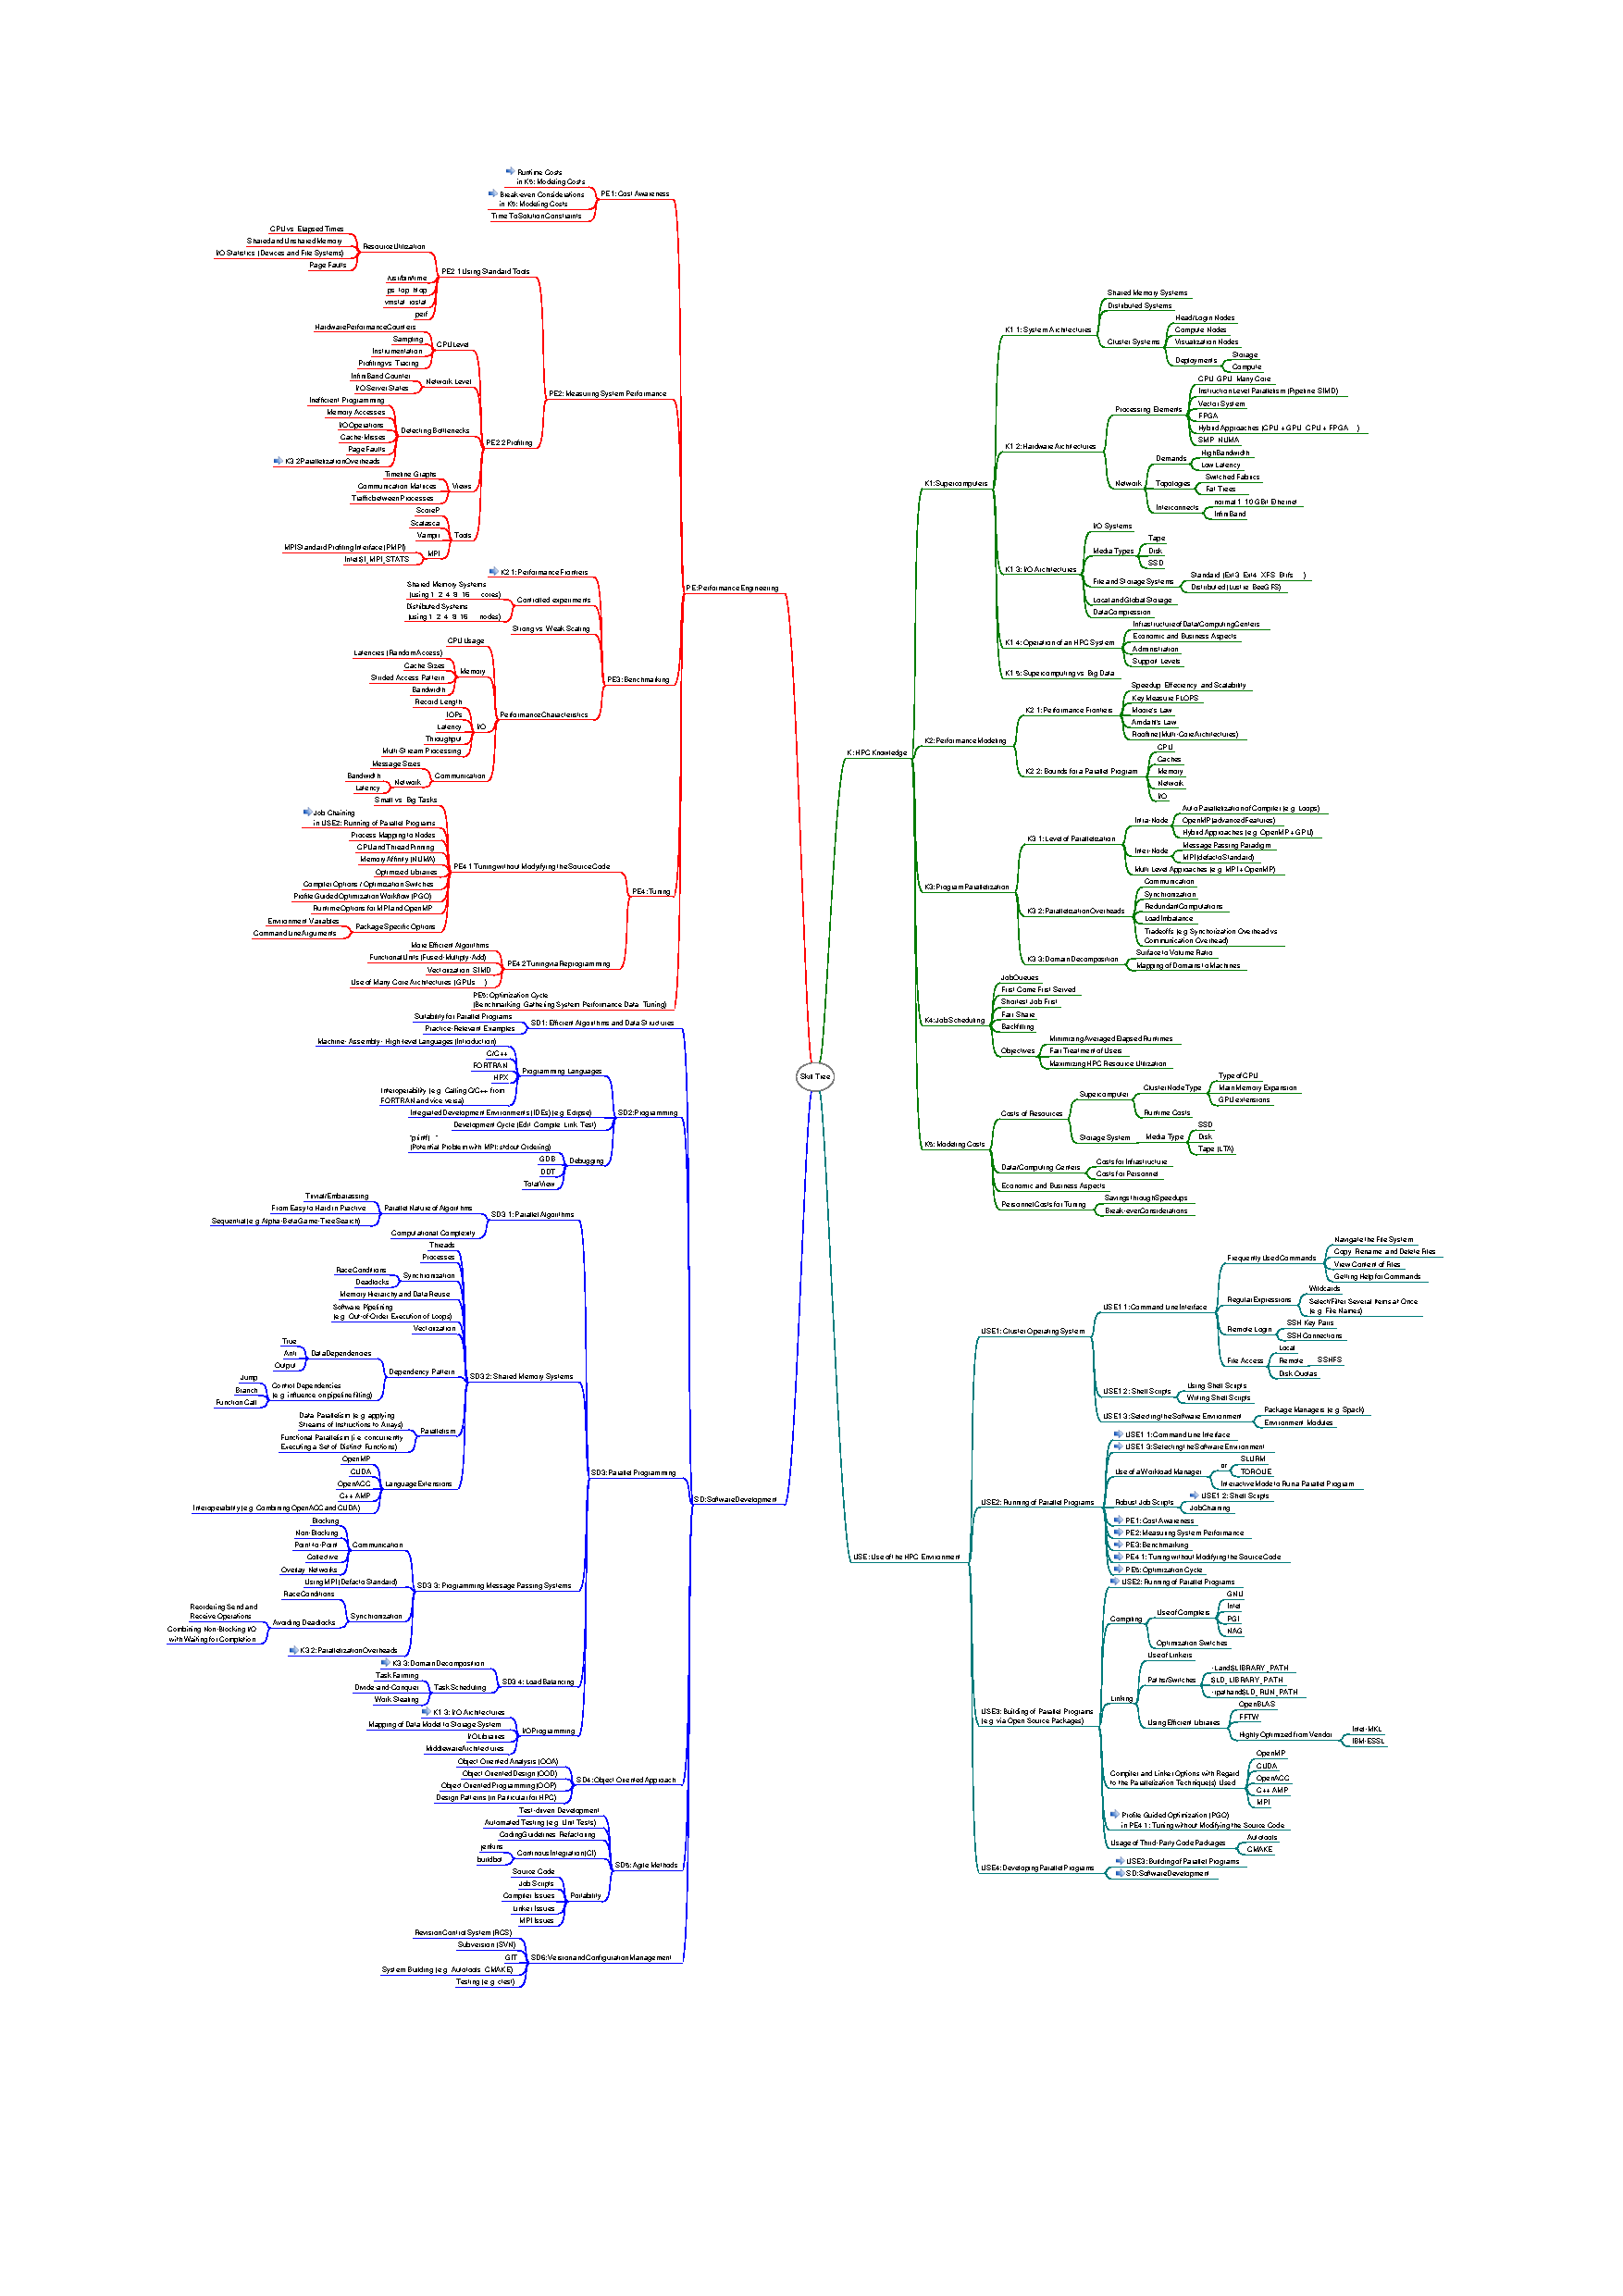
\includegraphics[width=15.0cm]{skill-tree}
	\caption{Top Level Competences with an expansion of PE4}
	\label{f_top_level_competences}
\end{figure*}

\subsection{Description of a skill}

Each skill on the tree and even the inner nodes are described in more detail as follows:

\begin{itemize}
  \item \textbf{ID}: ID according the organization in the skill tree. The last character indicates the level of the skill (Basic, Intermediate, or Advanced).
  \item \textbf{Name}: A speaking name for the skill.
  \item \textbf{Background}: Provides brief information motivating the need for the skill and how this skill fits into the skill tree; what is the bigger picture.
  \item \textbf{Aims}\footnote{The definition of aims and outcomes follows literature for higher education \cite{williamson2011good} and \url{https://www.heacademy.ac.uk/system/files/assessment-learning-outcomes.pdf}.}: They serve as broad purposes and are generally a statement of the intentions of the skill.
  They are not the statements of what a practitioner will learn or do.
  At a basic level, aims are trying to answer two questions: What is the purpose of this skill?
  What is the skill trying to achieve?
  \item \textbf{Learning outcomes (LOs)}: Defines briefly what what practitioners will know and learn.
  The objected are statements what prospect learners are able to do, they should
  describe or define an action be clearly stated be measurable/quantifiable to some extent by using action words.
\end{itemize}

On the leaf level, a skill is fine-grained and orthogonal to other skills -- we scope the level of detail here to be able to be taught in a 1.5 hour lecture up to a 4 hour workshop.
We believe this is a good granularity as it allows practitioners to cherry-pick the relevant skills and lecturers and examiners to prepare small lectures with well-defined content.
For technology-dependent skills on leaf level (e.g., a specific file system or workload manager), often introductory skills are provided that provide the foundation to many specialized skills each representing a specific hardware or software technology.

The aggregation within the tree is similar to the aggregation found in education as part of “individual teaching events”, “those specified for modules or short courses”, and “those specified for whole degree programmes” \cite{hussey2008learning}.
While that Hussey et al. conclude that LOs on the coarse grained level are not useful for high-level education, we use a similar concept, but relax the granularity/abstraction level of the learning outcome.

\subsection{Skill Examples}

Next, we present a generic skill that describes an inner-node in more details.
There is no actual delivery as a module or teaching event to deliver the content, it serves the purpose to inform the practitioner about the importance of the skill.

\begin{itemize}
  \item \textbf{ID}: USE4.2-B
  \item \textbf{Name}: Executing parallel applications
  \item \textbf{Background}:
  Parallel computers are operated differently than a normal PC, all users must share the system. Therefore, various operative procedures are in place. Users must understand these concepts and procedures to be able to use the available resources of a system to run a parallel application. Moreover, individual solutions can often be found in a specific system.
  \item \textbf{Aim}: To enable practitioners to comprehend the concepts and procedures for running parallel applications in HPC environments.
  To use the system to run and monitor the execution of parallel applications on the HPC system.

  \item \textbf{Learning outcomes}:
    \begin{itemize}
    \item explain the concepts and procedures for resource allocation and job execution in an HPC environment
    \item run interactive jobs and batch jobs
    \item comprehend and describe the expected behavior of job scripts
    \item change provided job scripts and embed them into shell scripts to run a variety of parallel applications
    \item analyze the output generated from a job scheduler and describe the cause of typically generated errors
    \end{itemize}
\end{itemize}

The next leaf-level skill describes how workload management works in general in HPC regardless of the specific software that implements such concepts.
It is intended that the aim and outcomes from the parent skill above are covered to some extend and refined into specifics.


\begin{itemize}
  \item \textbf{ID}: USE4.2.1-B
  \item \textbf{Name}: Workload manager introduction
  \item \textbf{Background}: There is a wide range of different workload managers in use. This skill covers generic and widely used concepts.
  \item \textbf{Aim}: To enable practitioners to comprehend and describe the basic architecture and concepts of resource allocation for an HPC system.
  \item \textbf{Learning outcomes}:

  \begin{itemize}
  \item comprehend the exclusive and shared usage model in HPC
  \item differentiate batch and interactive job submission
  \item comprehend the generic concepts and architecture of resource manager, scheduler, job and job script
  \item explain the role of environment variables as a means to communicate
  \item comprehend accounting principles
  \item explain the generic steps to run and monitor a single job
  \end{itemize}
\end{itemize}


The following skill describes a leaf-level skill for the usage of SLURM in the basic level.
While there is no formal dependency to the introduction (skill USE4.2.2-B), it is expected that practitioners have obtained the other skill before learning this one.

\begin{itemize}
  \item \textbf{ID}: USE4.2.2-B
  \item \textbf{Name}: SLURM Workload manager
  \item \textbf{Background}: SLURM is a widely used open-source workload manager providing various advanced features.
  \item \textbf{Aims}:
  \begin{itemize}
    \item To enable practitioners to use relevant tools to run and monitor parallel applications using SLURM.
    \item To enable practitioners to comprehend and describe the basic architecture of SLURM and the suite of tools.
  \end{itemize}
  \item \textbf{Learning outcomes}:
  \begin{itemize}
  \item run interactive jobs with salloc, a batch job with sbatch
  \item explain the architecture of SLURM, i.e., the role of slurmd, srun and the injection of environment variables
  \item explain the function of the tools: sacct, sbatch, salloc, srun, scancel, squeue, sinfo
  \item explain time limits and the benefit of a backfill scheduler
  \item comprehend that environment variables are set when running a job
  \item comprehend and describe the expected behavior of a simple job scripts
  \item comprehend how variables are prioritized when using command line and a script
  \item change a provided job template and embed them into shell scripts to run a variety of parallel applications
  \item analyze the output generated from submitting to the job scheduler and typically generated errors
  \end{itemize}
\end{itemize}

As you can see from the definition of the skill, these learning outcomes are focusing on the core needs to actually use SLURM effectively.
An intermediate skill could, e.g., add reservations.

%\begin{itemize}
%  \item \textbf{ID}:
%  \item \textbf{Name}:
%  \item \textbf{Background}:
%  \item \textbf{Aim}:
%  \item \textbf{Learning outcomes}:
%\end{itemize}


\section{Certification}

The certification


\begin{verbatim}
-----BEGIN PGP SIGNED MESSAGE-----
Hash: SHA512
HPC Certification Forum Certificate
This text confirms that "Julian M. Kunkel" has
successfully obtained the certificate
"The basic certificate" (id: 4711) at 02/2019.
Verification URL: https://hpc-certification.org/[...]
-----BEGIN PGP SIGNATURE-----
[...]
-----END PGP SIGNATURE-----
\end{verbatim}


\Cref{fig:awardedCertificate}


\begin{figure}
  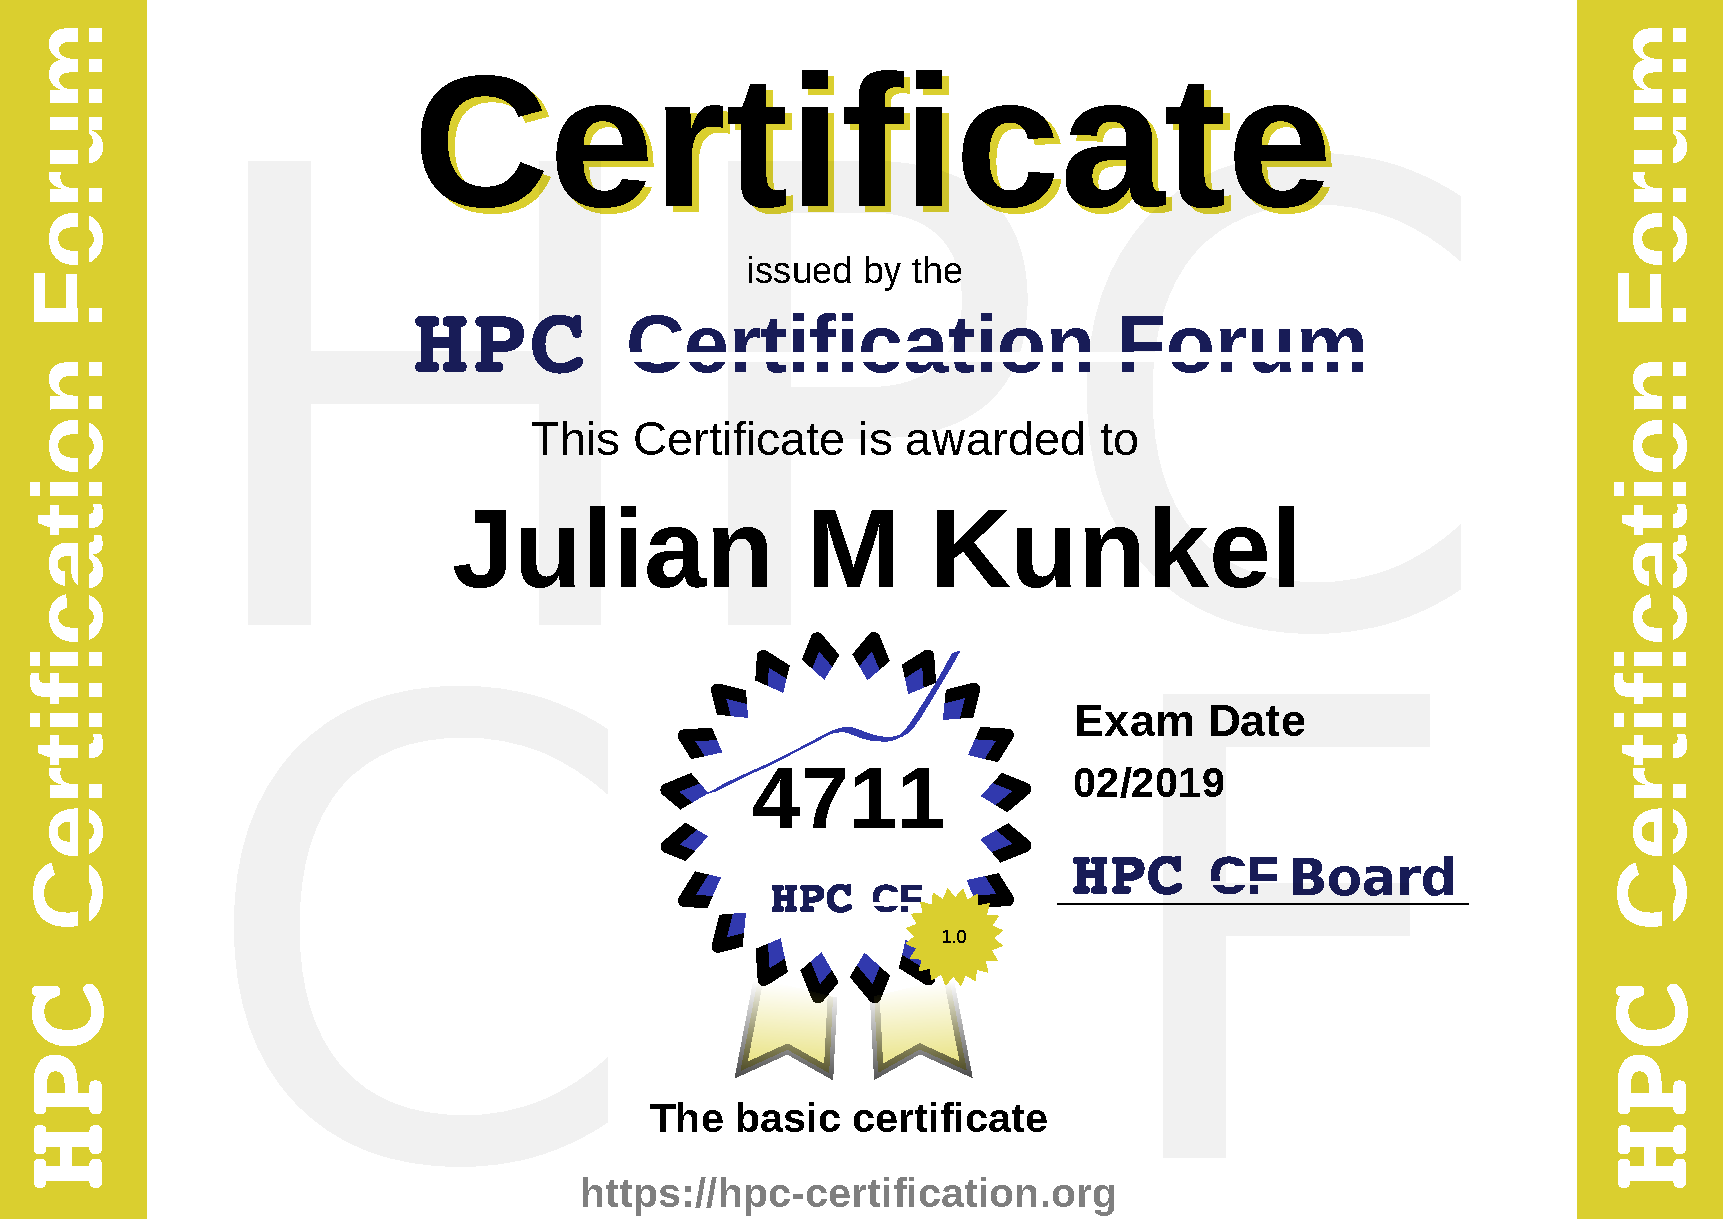
\includegraphics[width=0.48\textwidth]{JulianMKunkel}
  \caption{Draft for an awarded certificate}
  \label{fig:awardedCertificate}
\end{figure}


\subsection{Certificates}

\subsection{Examination Process}

A benefit of the fine-grained definition of learning outcomes is

\section{Ecosystem}

\section{Training Delivery}

The HPC Certification Forum is not developing training material directly or competing with providers of training material.
However, we support individuals and institutions by endorsing and promoting their training materials and courses in two ways.

Firstly, an author of training material is allowed to indicate on the training material itself or on promotional material the fact
which skills are covered by the material completely or partially.
We provide a seal that can be used for that purpose (see \Cref{fig:seal-teaching}).
The reference to the HPCCF and the seal can be used free of charge under the condition that the developer of the training material
registers a link to the material or course and their email address on our webpage using an online form.
That way, the HPCCF is informed about the usage of the seal.

Secondly, we will link on our webpage the endorsed training material for the individual skills and certificates.
By using JavaScript and dynamic webpage we will provide various views on the skills with and without links to suitable training materials.

Note that we are not intending to verify the correct usage of the skill explicitly.
However, in case the training material or course doesn't deliver the expected material practitioners may complain and we will remove the training material from our webpage.

We expect that this strategy will lead to the availability of good free training material for most skills
while companies and individuals can still charge for effective training courses.

\begin{figure}
  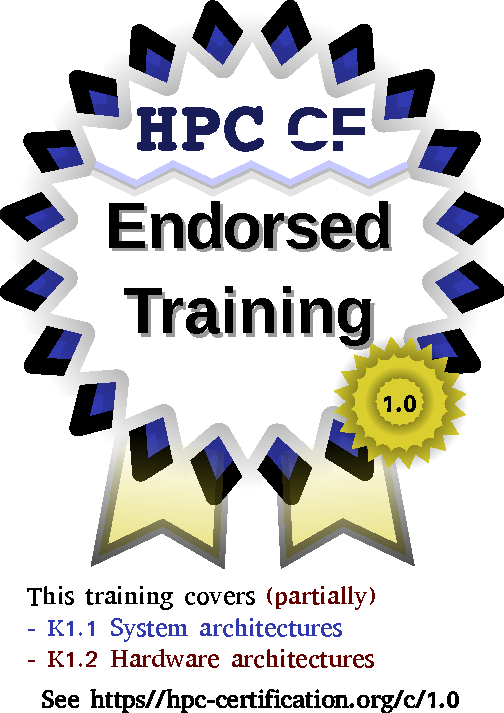
\includegraphics[width=0.3\textwidth]{certified}
  \caption{Draft for the seal for teaching material}
  \label{fig:seal-teaching}
\end{figure}


\subsection{Supportive Tools}

\section{Discussion of the Benefits}

Making clear what skills are required of or recommended for a competent HPC user would benefit both the HPC service providers and practitioners.
Moreover, it would allow centres to bundle together skills that are most beneficial for specific user roles and scientific domains.
From the perspective of content providers, existing training material can be mapped to competences allowing users to quickly identify and learn the skills they require.
Finally, the certificates recognized by the whole HPC community simplify inter-comparison of independently offered courses and provide additional incentive for participation.


\section{Related Work}
\jk{Please everyone!}

Relevant work can be classified into approaches to establish a curriculum or the creation of teaching material.
In academia, individual universities offer their own curriculum around scientific computing and HPC, covering theoretical aspects like the software development of numerical applications.
They are not tailored to the needs of a practitioner to actually use HPC systems effectively.
Data centers offer their own material and courses to support their own users.
Several projects address the generation and sharing of teaching material for HPC.
The EuroLab-4-HPC project establishes training in form of (online) courses\footnote{\url{https://www.eurolab4hpc.eu/}}.
The Barcelona Supercomputing Centre (BSC) aims to develop a professional training curriculum \cite{sancho2016bsc}.
The virtual organization XSEDE\footnote{\url{https://portal.xsede.org/web/xup/training/overview}} provides an online system to train the usage of an HPC system, structuring the corresponding information on their website into major topics like “Getting Started”.
The user can navigate the topics and receive further information.

\section{Conclusion}






\jk{Old stuff}


\subsection{Skills}

The skills represent competences in a fine-grained fashion.
A skill is defined by a unique key, short name, background, level, and a description of what it encompasses.
This model can be compared to the classification of school knowledge, for example, the skill with the short name "addition" could describe the math skill of being able to add numbers successfully.
The level serves the purpose of distinguishing the expertise further, a \textit{basic level}, for example, may mean to be able to add two numbers between 1-20 while the \textit{expert level} of that skill could indicate to be able to add any numbers.

The individual skills are organized into a tree that shows generic competences close to the root and refined skills on the leafs.
The two top-levels of the skill tree are shown in \Cref{f_top_level_competences}; we have identified more than 35 skills.
In respect to the granularity, we expect the basic level of a leaf like “Bash programming” can be acquired by novel users in a workshop day.
The tree serves the purpose of navigating across the skills, and at the same time a parent node defines the scope of its children.
For example, the \textit{USE} competence provides means of using the HPC environment to perform various tasks, such as running parallel applications, using core services of the operating system.
While the tree structure has been chosen as a graphical representation, some competences are cross-referenced, particularly in the skills of the USE branch.
The tree is managed in an XML file and we offer tools to visualize the skills as mindmap or embed them into a webpage.

\subsection{Certificates}

Certifying users with a certain competency is a core element of the program.
Since we identified so many skills, it is not useful to perform an exam on a single competence like “SLURM”.
Therefore, initially, we aim to group sets of skills into certificates and establish an online examination that attests users that they mastered a certain skill.
To be meaningful these tests must prevent cheating to some extent.
However, as any examination can be cheated with sufficient effort, we focus on practical aspects like a huge corpus of questions and some instantiated questions like \textit{how would you start ProgramX with 4 MPI processes?}




\appendix

\begin{acks}
\small
This work was supported by the German Research Foundation (DFG) under grants LU 1353/12-1, OL 241/2-1, and RI 1068/7-1.
\end{acks}

\bibliographystyle{ACM-Reference-Format}
\bibliography{bibliography}

\end{document}
